\section{Quantity and Money}
\label{sec:quantity}
\code{Quantity} is used to represent amounts of anything.
Three attributes allow \code{Quantity} to specify everything: a numerical value (\code{BigDecimal}), a (measurement) unit or metric (\code{Metric}), and a type specifying the rounding of the numerical type (\code{RoundingStrategy}), as can be seen in Figure \ref{quantity_overview}.

\code{Quantity} objects are immutable and the class implements the \code{Comparable} interface.

\begin{figure}[ht]
	\centering
  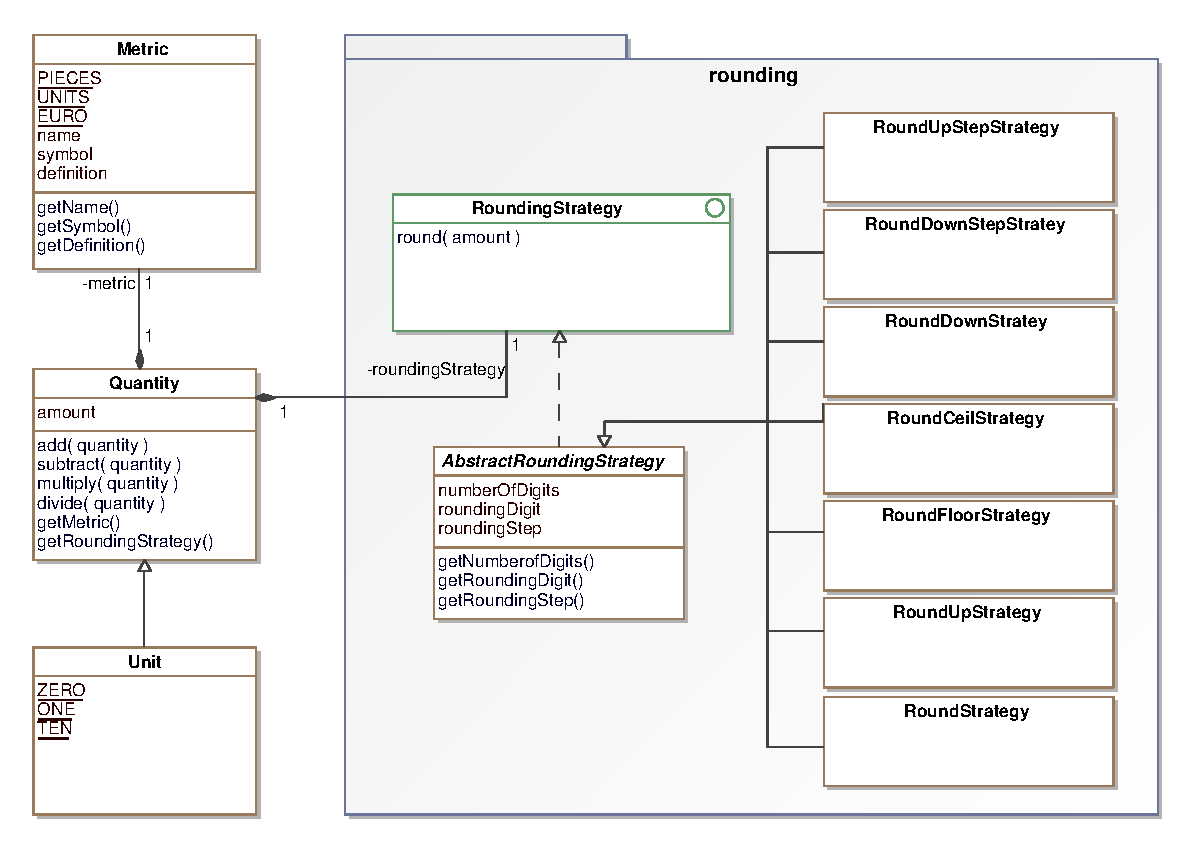
\includegraphics[width=1.0\textwidth]{images/Quantity_Overview.eps}
	\label{quantity_overview}
	\caption{Quantity - Class Overview}
\end{figure}

\subsection{\code{BigDecimal} - Representing numerical values}
\code{BigDecimal} was chosen as datatype for the \code{amount} attribute (see Figure~\ref{quantity_overview}) over \code{float} or \code{double} because of its arbitraty precision.
Moreover, objects of \code{BigDecimal} are immutable and the \code{BigDecimal} class provides operations for including, but not limited to: arithmetic, rounding, and comparison.

\subsection{\code{Metric} - What is represented}
The composite type \code{Metric} contains all information pertaining to the unit or metric of the represented object.
Examples for units or metrics are: m (meter), s (second), pcs (pieces).
For example consider the unit of length "meter": represented by an object of the class \code{Metric} the symbol would be set to "\code{m}" and the name to "\code{meter}".
Furthermore, an object of type \code{Metric} has a description field, to explain the meaning of the metric in detail.
For the example of a meter a possible description could be "\code{The meter is the length of the path travelled by light in vacuum during a time interval of 1/299 792 458 of a second.}".

Convenience instances exist for euros, pieces and units, namely \code{EURO}, \code{PIECES}, and \code{UNIT} (see Figure \ref{quantity_overview}).

%\subsection{\code{RoundingStrategy} - How to handle half a person}
%When handling quantities of unkown metric, standard rounding rules cannot always be employed.
%The case of natural persons is just one example, when rounding rules have to be restricted to yield a useful result.
%You can round in four general directions: away from zero (\code{RoundUpStrategy}), towards zero (\code{RoundDownStrategy}), towards positive infinity (\code{RoundCeilStrategy}), and towards negative infinity (\code{RoundFloorStrategy}).

%Additionally, you can specify the digits after the decimal delimiter (\code{numberOfDigits} in Figure~\ref{quantity_overview}).
%Monetary values in \euro{} or \$US are often just represented with two digits after the decimal delimiter.
%Other values, such as kilo grams may be required to be specified to four digits after the decimal delimiter or even more.
%In case of (natural) persons, the digits after the decimal delimiter is usually zero, except you are working in statistics (1.45 children per couple) or you are a serial killer dismembering your victims.\footnote{Of course you can only kill an integral number of people. However, only a part of a victims body may be found. Anyway, in case you have not noticed: that was a joke. Haha. Fat chance.}

%The third parameter for rounding is the rounding digit, i.e. the number specifying when you round up or down.
%Usually, this number is five, but it can be specified using the attribute \code{roundingDigit} and the \code{RoundStrategy} as strategy.
%In case of persons, it is one: if you have $n.0\,persons$, you round down, otherwise up.
%If you are calculating a capacity for persons, you will have to round down.
%This can be achieved by specifying the correct rounding direction.
%\\

\subsection{Rounding}
Rounding is an arithmetic operation where a numberical value is replaced by another, simpler representation.
Rounding is often results in a number which is easier to handle than the original value, for example $3.1415$ instead of $\pi$, or $1.1414$ instead of $\sqrt{2}$.
Also, rounding may be employed to indicate the accuracy of a computed or measured value. 
For example a value is calculated to be $3.4563$ but it is known the result is only accurate to one hundredth because of measurement errors, so the result may be rounded to $3.46$. 
Rounding may also be used to limit the number of significant digits, for example in statistics.
The german population is rounded to full thousands by the Federal Statistical Office and the statistical Offices of the L\"ander\footnote{\url{http://www.statistik-portal.de/Statistik-Portal/en/en_zs01_bund.asp}}.
\\

Different types of rounding exist. A number can be rounded to a specific precision, to an (integer) multiple of a step or increment, or to the nearest available value ot of a set of preferred values.
Thus, rounding is implemented as strategy pattern, allowing a consistent interface to be used with different algorithms.
So far, the only strategy implemented is the \code{BasicRoundingStrategy} which supports rounding to a specific precision or rounding to a multiple of a pre-determined multiple of a step.
\\

Rounding to precision zero is also known as rounding to integer.
%When doing so, five general strategies, as outlined in Table \ref{roundstrat} can be employed.
When doing so, five general strategies can be employed:

\begin{itemize}
\item{\textbf{up} - result is the next integer, away from zero}
\item{\textbf{down} (also known as ``truncation'') - result is the next integer, towards zero}
\item{\textbf{ceil} - result is the next integer, towards positive infinity}
\item{\textbf{floor} - result is the next integer, towards negative infinity}
\item{\textbf{half} - result is the nearest integer}
\end{itemize}

%\begin{table}
%\begin{tabular}{c}
%oo \\
%foo \\
%\end{tabular}
%\caption{\label{roundstrat}foo-table}
%\end{table}

All strategies except the last yield unambiguous results.
If a number ends in $x.5$ and is rounded to the nearest integer two results exist: $x$ and $x+1$, since both have the same absolute difference to $x.5$.
To resolve the ambiguity, tie breaking rules have to be employed.
The first four strategies to round integers (up, down, ceil, floor) can also be used for tie-breaking.
Additionally, more sophisticated methods may be employed, for example:

\begin{itemize}
\item{\textbf{even} - result is the nearest even integer}
\item{\textbf{odd} - result is the nearest odd integer}
\item{\textbf{stochastic} - result randomly chosen to be $x$ or $x+1$}
\item{\textbf{alternate} - using strategies up and down intermittently}
\end{itemize}

A technique called dithering, which is related to stochastic rounding tie-breaking rule, is used when instead of the accuracy of single rounding operation is less important than the distribution of rounding results across a set of values.
Dithering is often used in quantizing image or audio data.
For example, if a continous stream of values of approximately $0.88$ should be rounded to zero digits after the radix delimiter, that is to integer, would result in contiuous $1$ or $0$ result, depending on the strategy.
Using dithering, a number is rounded up (or down) with the probability of the fraction.
In our example, this would result in a stream containing $88\%$ ones and $12\%$ zeroes, randomly distributed.
A similar technique, which reduces the average error, is called ``error diffusion''.

As mentioned earlier, only one strategy is implemented as of yet, namely \code{BasicRoundingStrategy}.
Instantiating an object of this strategy, it is possible to specify either a rounding step or a precision in digits after the radix delimiter.
Internally, the following algorithm is used to round numbers:
\begin{equation*}
x = round(q/m) * m
\end{equation*}
where $q$ is the number to be rounded, $m$ is the increment or rounding step, $x$ is the result, and $round$ is a rounding strategy to round the quotient $q/m$ to an integer value.

When the number of digits after the radix delimiter are specified, the appropriate rounding step is calculated as follows:
\begin{equation*}
step = \frac{1}{10^{digits}} = 10^{-digits}
\end{equation*}

For example, rounding a number to four digits after the radix delimiter is equal to rounding the number to the next (integer) multiple of $0.0001$.

Rounding to a nearest step or increment, can be used if something is sold in fixed quantities.
For example, if an item is sold in packs of $50$, and someone punches in $40$, you will have to round up to $50$.
So your rounding step is $50$.
Another example is material, which is sold by the meter or yard.
You have to round the amount specified by your customer accordingly.
Of course, a rounding step can be smaller than $1$, i.e. $0.25$.
\\

Two convenience rounding strategies exist so far: \code{RoundingStrategy.MONETARY} rounding with four digits after the decimal delimiter and rounding towards zero, and \code{RoundingStrategy.ROUND\_ONE} with zero digits after the decimal delimiter and also rounding towards zero.
\\

Rounding strategies which are not yet implemented, but may be interesting to \salespoint{} users and developers are scaled rounding, rounding to nearest value of a predetermined set and a sum preserving rounding strategy.
Implementing these strategies may require extending the \code{RoundingStrategy} interface.

Scaled rounding is used to round values on a logarithmic scale.
Near zero a high precision is required, for example using three digits after the radix delimiter.
But farther away precision requirements drop, so only one digit after the radix delimiter may suffice.
Thus, the precision to which is rounded depends on the magnitude of the value to be rounded.

Rounding to nearest preferred value is used, when a calculated value is rounded to the nearest standard value.
Examples of preferred values are the E series, the Renard series, powers of two, metric paper sizes and pen sizes, tuning systems in music, or film speed, aperture sizes and shutter speeds in photography.
E series are most commonly used in electronics industry for resistor, capacitor, and inductor values.\footnote{IEC 60063}
In computer science, powers of two are often used as preferred values for sizes.
Paper is sized so that neighboring dimensions have a ratio of $\sqrt2$.\footnote{ISO 216}
This also applies for pen sizes, so that a pen size is available for a scaled drawing.

Sum preserving rounding is necessary if, for example for every item on an invoice the tax is explicitly listed.
The tax for each item has to be rounded, introducing a rounding error.
When the taxes for each item are summed up, the sum has to match the tax calculated for the summed prices of all items.
This is seldomly the case, so the rounding of the individual tax has to be fitted.
The method of least squares may be used to achieve fitting.
Another algorithm which may be used is minimizing the round-off error.

\subsection{\code{Money} - A usecase for \code{Quantity}}
An object of the class \code{Money} is used to represent an amount of currency.
The following paragraphs detail the intended use, internal modelling and implementation of \code{Money}.
The UML model is given in Figure \ref{money_overview}.

\begin{figure}[ht]
	\centering
  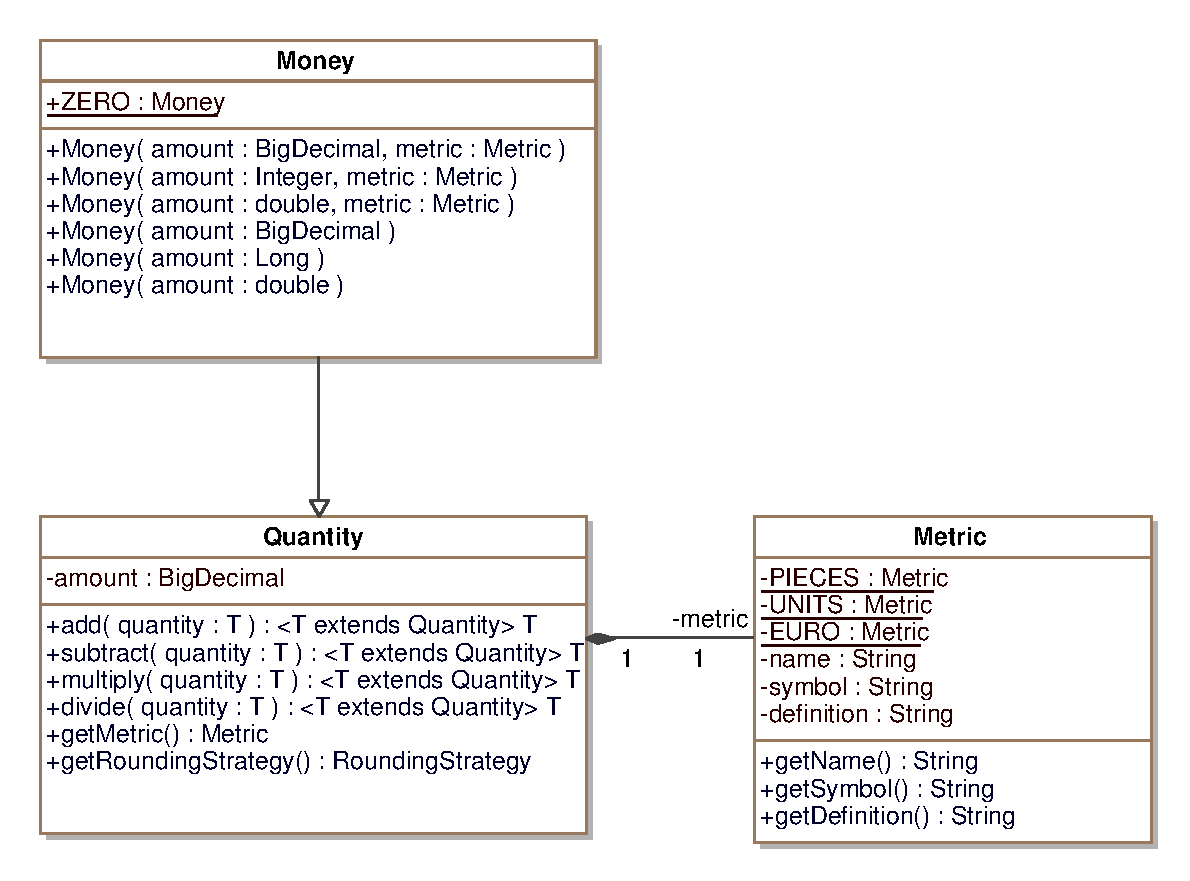
\includegraphics[width=0.75\textwidth]{images/Money_Overview.eps}
	\label{money_overview}
	\caption{Money - Class Overview}
\end{figure}

A \code{Money} object can be instantiated by passing the numerical value as constructor parameter.
In this case, the metric \code{Metric.EURO} is used, as well as \code{RoundingStrategy.MONETARY} for the rounding strategy attribute.

For other currencies, a \code{Metric} parameter can be passed to the constructor along with a numerical paramter.
However, conversion between currencies is not supported, as it was not deemed necessary.

The rounding strategy cannot be overridden.
Internally, \code{Money} objects use four digits after the decimal delimiter for arithmetic operations to minimize the rounding error.
The \code{toString()} method, however, limits the output to the expected two digits after the decimal delimiter and appends the symbol of the associated \code{Metric}.

Two convenience instances exist: \code{Money.ZERO}, representing \euro{0,00}, and \code{Money.OVER9000}, representing an amount greater than \euro{9000,00}.

\subsection[]{\code{Unit} - Representing persons or other integral\protect\footnote{whole-number} items}
To represent integral items conveniently, the objects of class \code{Unit} can be used.
The rounding strategy is fixed for all instances to \code{RoundingStrategy.ROUND\_ONE} (Figure~\ref{quantity_overview}) and \code{Metric.PIECES} (Figure~\ref{money_overview}) is used as metric.
Convenience instances for amounts of zero, one and ten unit(s) exist (\code{Unit.ZERO}, \code{Unit.ONE}, and \code{Unit.TEN}; see Figure~\ref{quantity_overview}).
